\documentclass{article}
\usepackage[utf8]{inputenc}
\usepackage[T1]{fontenc}
\usepackage[polish]{babel}
\usepackage{graphicx}
\usepackage{pdfpages}
\graphicspath{ {./charts/} }
\usepackage{minted}
\usepackage[a4paper,top=2cm, total={6in, 8in}]{geometry}
\renewcommand{\contentsname}{Spis treści}

\title{Biblioteka arytmetyki liczb stałoprzecinkowych dowolnej precyzji z wykorzystaniem wewnętrznej reprezentacji U2.}

\author{Leszek Błażewski \\ \\Karol Noga}

\date{Semestr letni 2018/2019}

\begin{document}
\maketitle
\thispagestyle{empty}
\clearpage
\setcounter{page}{1}
\tableofcontents
\newpage{}

\section{Założenia projektowe}

Celem projektu była implementacja biblioteki oferującej podstawowe operacje arytmetyczne na liczbach dowolnej precyzji, która wykorzystuje system uzupełnień do dwóch jako bazowy. Jednym z wymagań projektowych było zapewnienie możliwe najszybszej oraz najbardziej optymalnej implementacji danych algorytmów wykorzystując do tego celu instrukcje procesora. Dalsza część projektu obejmowała sprawdzenie poprawności zaimplementowanych operacji oraz przeprowadzenie testów wydajnościowych. Ostatnim etapem była analiza napisanego kodu przy pomocy narzędzi oferujących funkcje pozwalające na zmierzenie wydajności danych kawałków kodu, profilowanie oraz analizę dotyczącą zarządzania pamięcią.

\section{Technologie i narzędzia}

Rozdział ten traktuje o argumentach, które skłoniły nas do wyboru danego języka oraz zawiera krótki opis narzędzi i technologi, które wykorzystaliśmy w projekcie.

Cały projekt wraz z dokumentacją dostępny jest w publicznym repozytorium, które dostępne jest pod poniższym linkiem:

\begin{center}
\textbf{https://github.com/dex1g/OiAK}
\end{center}{}

\subsection{Wybrany język}

Zdecydowaliśmy się na implementację biblioteki w języku $C$, ponieważ kod programu kompilowany jest do kodu natywnego, dzięki czemu algorytmy pisane w tym języku przy odpowiedniej implementacji są wydajniejsze niż te pisane w językach interpretowanych oraz uruchamianych na maszynach wirtualnych. Kolejnym powodem wyboru tego języka jest łatwość integracji instrukcji mikroprocesora z kodem pisanym w tym języku oraz możliwość bezpośredniej deasemblacji kawałków kodu pisanych w $C$. Kluczowa jest również pełna kontrola programisty nad alokowaną pamięcią programu, co przekłada się na wydajność pisanych algorytmów. Zdecydowaliśmy się pisać całą aplikację na architekturę 32 bitową, ponieważ mamy z nią styczność na laboratoriach i wykładzie oraz znaliśmy już podstawowe założenia \textit{ABI}, dzięki czemu cała implementacja przebiegła sprawniej.

\subsection{Wykorzystane narzędzia}

Bibliotekę staraliśmy się tworzyć w konwencji Test Driven Deployment, dzięki czemu każdy algorytm pokryty jest serią testów, która sprawdza większość możliwych przypadków oraz poprawność implementacji. Do realizacji tego zadania posłużyliśmy się biblioteką $Unity$, która oferuje bogaty zestaw funkcji pozwalających na asercję wybranych danych po przeprowadzeniu odpowiednich działań.. Podczas profilowania posłużyliśmy się narzędziem $Gprof$, które pozwoliło nam na dynamiczną analizę kodu programu oraz wykrycie funkcji, które wymagają refaktoryzacji oraz optymalizacji. Ostatnim użytym narzędziem był $Valgrind$, który dostarczył informacji o błędnym zarządzaniu pamięcią.  Do projektu dodano również automatyczne budowanie testów jednostkowych przy każdej zmianie w repozytorium, zrealizowane przy pomocy platformy $Travis$ $CI$. Poniżej zamieszczono listę wykorzystanych narzędzi wraz z ich zastosowaniem.

\clearpage

\begin{itemize}
    \itemsep0em 
    \item $gcc$ - Kompilacja oraz optymalizacja
    \item $Unity$ - biblioteka użyta to implementacji testów jednostkowych
    \item $Gprof$ - profilowanie
    \item $Valgrind$ - analiza wykorzystanej pamięci
    \item $Git$ - system kontroli wersji
    \item $Travis$ $CI$ - automatyczne budowanie projektu
\end{itemize}

\section{Opis funkcjonalności biblioteki}

Biblioteka oferuje cztery podstawowe operacje arytmetyczne: dodawanie, odejmowanie, mnożenie oraz dzielenie. Wszystkie operacje wymagają argumentów w formacie, który został stworzony specjalnie na potrzeby odpowiedniej reprezentacji liczb w języku $C$, w związku z czym biblioteka oferuje również zestaw funkcji pozwalający na konwersję zadanej liczby z systemu szesnastkowego na wymagany. Dodatkowo dodano możliwość odczytu danych z pliku tekstowego zawierającego liczbę szesnastkową lub bezpośrednio z pliku binarnego.

\section{Wykorzystanie biblioteki}

Rozdział ten zawiera informacje, które pozwalają zaimportować bibliotekę do projektu oraz sposób przeprowadzenia testów.

\subsection{Dołączenie biblioteki do projektu}

Aby skorzystać z wszystkich funkcji oferowanych przez bibliotekę do projektu dołączyć należy wszystkie pliki znajdujące się w folderze $src$. Następnie w plikach programu zaimportować należy pliki nagłówkowe oraz podczas kompilacji załączyć odpowiadające im pliku źródłowe oraz plik z kodem asemblerowym, które zawierają algorytmy danych operacji zrealizowane przy pomocy instrukcji procesora.

Podczas wykorzystania funkcji pamiętać należy, że wszystkie argumenty każdej z operacji są dealokowane w trakcie procesu obliczania wyniku danego działania, dlatego wskaźnik na tablicę zawierającą liczbę znajdujący się w obiekcie struktury \textit{TCNumber} musi wskazywać na tablicę, która alokowana była dynamicznie. Gdy chcemy wykorzystać funkcje dla tablic statycznych musimy wcześniej wykorzystać funkcję \textit{createTCNumber}, która zaalokuje wymagany obszar i przepisze do niego zawartość liczby, lecz należy liczyć się z ograniczeniami dotyczącymi dostępnej pamięci operacyjnej programu w architekturze 32-bitowej.

\subsection{Wykonanie testów jednostkowych i wydajnościowych}

Dokładny opis implementacji danych testów jednostkowych oraz wydajnościowych zamieszczony został w rozdziale \ref{Implementacja}. Poniżej zamieszczono natomiast sposób wykonania danych testów.

W celu sprawdzenia czy wszystkie oferowane funkcje spełniają swoje zadania, istnieje możliwość wykonania wszystkich testów jednostkowych, które zapewniają pełne pokrycie wszystkich implementacji.
Aby wykonać testy wystarczy wykonać poniższą komendę z głównego folderu projektu:

\begin{minted}{bash}
# Run all unit tests
cd tests/ && make AllTests
\end{minted}

Natomiast w celu wykonania testów wydajnościowych w pierwszej kolejności wygenerować należy dane testowe, przy czym zalecanym narzędziem jest $dd$ dostępne na systemach $Unixo$ podobnych. Do repozytorium dodany został skrypt \textit{generateData.sh} znajdujący się w folderze \textit{data/}, który automatycznie wygeneruje potrzebne pliki. Poniżej zamieszczono kolejne komendy pozwalające na wygenerowanie odpowiednich danych oraz wykonanie testów wydajnościowych. Dane testowe nie zostały dołączone do projektu, ponieważ wiele plików posiada znaczne rozmiary, przez co nie mogą być one przetrzymywane w repozytorium.

\begin{minted}{bash}
# move to data directory
cd efficiencyTests/data
# Provide executive privileges
chmod +x ./generateData.sh
# Generate data using dd tool or provided script
./generateData.sh
# Move to the efficiencyTests directory and run the tests
cd ../ && make EfficiencyTests
\end{minted}



\section{Opis struktury projektu}

Cały projekt podzielony został na cztery zasadnicze foldery: 
\begin{itemize}
    \item documentation
    \item efficiencyTests
    \item src
    \item tests
\end{itemize}

Poniżej zamieszczono krótki opis każdego z folderów oraz jego zawartości.

\subsection{documentation}

Folder zawiera sprawozdania w formacie $.tex$, które sukcesywnie oddawane były na kolejnych zajęciach projektowych. Prezentują one cały proces rozwoju naszego projektu oraz pokazują kolejne implementacje oraz modyfikacje algorytmów. W folderze zamieszczono również sprawozdanie z całego projektu.

\subsection{efficiencyTests}

Folder składa się z plików realizujących testy wydajnościowe zaimplementowanych algorytmów oraz zawiera poprzednie wersje operacji arytmetycznych umieszczone w podfolderze \textit{PastImplementations}, które są znacznie mniej wydajne od funkcji zawartych w bibliotece. Postanowiliśmy pozostawić te implementacje w celu pokazania różnicy czasów wykonywania obu algorytmów w zależności od implementacji. W folderze tym znajduję się również folder $data$, który przechowuje wszystkie potrzebne pliki do przeprowadzenia testów. W tym folderze przeprowadzane jest również profilowanie kodu, którego rezultat znajduje się w \textit{pliku profile-data.txt}.

\subsection{src}

Folder zawiera główne pliki biblioteki, gdzie umieszczone zostały najbardziej wydajne i optymalne implementacje stworzone w trakcie realizacji projektu. W celu zapewnienia poprawności działania dołączanej biblioteki wszystkie pliki z tego folderu powinny być załączane do danego projektu.

\subsection{tests}

Folder zawiera wszystkie testy jednostkowe, które podzielone zostały ze względu na sprawdzane treści: \textit{ArithmeticOperationsTests.c} oraz \textit{ParsersTests.c}. W folderze znajduje się również plik \textit{Makefile} w którym zdefiniowano komendy przyśpieszające budowę oraz egzekucję danych testów. Folder \textit{Unity} zawiera kod źródłowy biblioteki dostępnej na licencji MIT, której użyliśmy do realizacji testów jednostkowych.

\section{Implementacja} \label{Implementacja}

W tym rozdziale zamieszczono dokładny opis zaimplementowanych funkcji wraz z wycinkami kodu, które wymagają komentarza oraz realizują kluczowe funkcje biblioteki. Kod źródłowy również zawiera komentarze, które tłumaczą sposób rozwiązania danego problemu. 

Podczas implementacji wszystkich algorytmów staraliśmy się możliwie często wykorzystywać funkcje udostępniane z poziomu języka \textit{C}, aby wykorzystać możliwości optymalizacyjne udostępniane przez kompilator \textit{gcc}. Niestety w wielu przypadkach nie istnieją gotowe moduły w języku \textit{C} pozwalające na bezpośredni dostęp do instrukcji procesora w związku z czym zdefiniowaliśmy własne funkcje w celu zwiększenia wydajności danych algorytmów.

\subsection{Sposób reprezentacji liczb}

Aby zapewnić dowolną precyzję liczb podczas wykonywanych operacji stworzyliśmy własną strukturę, która pozwala na realizację tego wymagania.

\begin{minted}{C}
typedef struct
{
    unsigned char *number;
    unsigned int numberSize; // bytewise
    int numberPosition;      // bitwise
} TCNumber;
\end{minted}

Pole \textit{number} jest wskaźnikiem na tablicę charów, która przechowuje liczbę w postaci bajtowej, gdzie liczba reprezentowana jest w systemie U2.

Pole \textit{numberSize} przechowuje długość liczby w reprezentacji bajtowej, ponieważ w języku \textit{C} tablice nie pamiętają swojego rozmiaru.

Natomiast pole \textit{numberPosition} odpowiada za przechowywanie wartości, która określa pozycję najmniej znaczącego bitu liczby.

\clearpage

\subsection{Odczyt liczby}

Do biblioteki załączyliśmy również dwie funkcje odpowiedzialne za tworzenie nowego obiektu struktury \textit{TCNumber}. Funkcja bez realokacji tablicy znacząco zwiększa wydajność algorytmów  i pozwala na zaoszczędzenie znacznych ilości pamięci. Aby odciążyć użytkownika z dealokacji dodaliśmy również funkcję, która poprawnie zwalnia daną liczbę. Wszystkie operacje dealokują argumenty podawane do funkcji aby zaoszczędzić możliwe jak największą ilość pamięci. Dlatego biblioteka posiada dwa rodzaje inicjalizacji obiektów, aby pozwolić na stosowanie operacji zarówno dla tablic znajdujących się na stosie oraz tych alokowanych dynamicznie.

Do wczytywania liczby z standardowego wejścia posłużyliśmy się funkcją \textit{scnaf} z specjalną flagą dostępną w standardzie POSIX, która alokuje wymagany obszar do wczytania liczby. Aby zapewnić również zgodność z systemami nie wspierającymi standardu POSIX dodaliśmy funkcję, która odczytuje liczbę z pliku binarnego.

\subsection{Konwersja}

Biblioteka oferuje funkcję pozwalającą na konwersję z systemu szesnastkowego, gdzie liczba zapisana jest jako ciąg znaków \textit{ASCII} na system \textit{U2}. Pierwszym etapem konwersji jest ustalenie znaku konwertowanej liczby, wyliczenie jej długości oraz pozycji najmniej znaczącego bitu liczby. Następnie wykorzystujemy funkcję $asciiToByte$, która w zależności od danego znaku szesnastkowego konwertuje go na odpowiednią mu reprezentację bajtową. Następnie posługujemy się przesunięciem bitowym w lewo w celu zachowania poprawnej wartości konwertowanego znaku. Jeśli liczba jest ujemna w ostatnim kroku algorytmu negujemy każdy z bitów a następnie dodajemy do zanegowanej liczby jedynkę, uzyskując w ten sposób reprezentację liczby w systemie \textit{U2}.

\subsection{Operacja arytmetyczne}

Poniżej znajduje się opis każdego z algorytmów wraz z kawałkami kodu, które obrazują sposób realizacji danego zagadnienia oraz komentarze wyjaśniające daną implementację.

Każda z funkcji napisana została jako odpowiednia metoda w języku \textit{C}, która realizuje wszystkie potrzebne operacje do odpowiedniego przygotowania argumentów oraz wyniku do operacji, natomiast sam algorytm został napisany w języku asembler w celu zwiększenia wydajności oraz wykorzystania instrukcji procesora.

Wszystkie funkcje, które korzystają z mnemoników, zawierają w sobie szereg operacji służących zapewnianiu zgodności z \textit{ABI}, dzięki czemu biblioteka zapewnia pełną integrację wykonywanych operacji z systemem operacyjnym na którym wykonywany jest kod programu oraz pozwala na zaawansowaną kompilację z użyciem \textit{gcc}.

\clearpage

\subsubsection{Dodawanie}

Pierwszym etapem dodawania jest wyznaczenie rozmiaru wyniku, który w przypadku operacji dodawania jest o jedną pozycję większy od większego z argumentów, ponieważ uwzględnić należy ewentualne przeniesienie na najwyższą pozycję.

\begin{minted}{C}
long long highestPos = addend1->numberPosition + (long long)addend1->numberSize * 8;
if (addend2->numberPosition + (long long)addend2->numberSize * 8 > highestPos)
    highestPos = addend2->numberPosition + (long long)addend2->numberSize * 8;
int lowestPos = addend1->numberPosition;
if (addend2->numberPosition < lowestPos)
    lowestPos = addend2->numberPosition;
unsigned int resultSize = (highestPos - lowestPos) / 8 + 1;
\end{minted}

Rzutowanie na zmienną typu \textit{long long} jest konieczne, ponieważ dla wielkich liczb pozycja może przyjmować wartości które nie zmieszczą się w zmiennej \textit{int}. Należy pamiętać, że pozycja liczb liczona jest bitowo natomiast wielkość wyniku określana jest w bajtach.

W kolejnym kroku wyliczamy pozycję najbardziej znaczącego bitu drugiej liczby względem pierwszej, ponieważ jedynie pierwsza liczba skalowana jest do rozmiaru wyniku. Wyliczony indeks wykorzystany jest w algorytmie do poprawnej propagacji przeniesienia na pozycje wyższe od pozycji najbardziej znaczącego bitu drugiej liczby.

Następnie skalujemy pierwszy z argumentów do rozmiaru wyniku, ponieważ w nim zapisywany będzie wynik operacji. Operacja skalowania danej liczby do zadanego rozmiaru została dokładnie opisana w rozdziale \ref{Skalowanie liczby}.

Później sprawdzamy bit rozszerzenia drugiego z operandów i gdy wynosi on jeden, od pierwszego składnika dodawania odejmujemy jedynkę na pozycji znajdującej się o jedną pozycję wyżej od najbardziej znaczącego bitu drugiej liczby. Operacja ta jest konieczna w celu zapewnienia poprawnej propagacji przeniesienia gdy drugi z operandów jest ujemny.

Następnie odpowiednie zmienne przekazujemy do funkcji \textit{array\_adc}, która wykorzystuje instrukcje procesora do obliczenia wyniku. Należy zauważyć, że instrukcja \textit{cmp} wpływa na flagę przeniesienia, przez co nie może zostać użyta do sprawdzania warunku końca pętli. W celu zachowania poprawnej wartości flagi przeniesienia podczas kolejnych iteracji pętli posłużyliśmy się kombinacją instrukcji \textit{dec} oraz \textit{jns}, które nie powodują zmiany stanu flagi, jednocześnie gwarantując poprawną ilość obiegów pętli. Na końcu zwracamy pierwszy z argumentów, w którym zapisany jest wynik całej operacji.

\subsubsection{Odejmowanie}

Operacja odejmowania została zrealizowana analogicznie do algorytmu dodawania, z tym że wykorzystana została instrukcja \textit{sbb} oraz pętla służąca do odpowiedniej propagacji pożyczki na pozycjach odjemnej wyższych od pozycji najbardziej znaczącego bitu odjemnika została przedefiniowana aby zapewnić poprawną propagację.

Zmianie uległa też operacja, która wykonywana jest w przypadku ujemnej wartości drugiego operandu. Gdy odjemnik jest ujemny, do odjemnej dodajemy jedynkę na pozycji znajdującej się o jedną pozycję wyżej od najbardziej znaczącego bitu odjemnika, aby poprawnie propagować przeniesienie podczas wyznaczania wyniku.

\subsubsection{Mnożenie}

Pierwszym etapem mnożenia jest wyznaczenie rozmiaru wyniku, który równy jest sumie rozmiarów mnożnej i mnożnika. Natomiast pozycja najmniej znaczącego bitu iloczynu równa jest sumie pozycji najmniej znaczących bitów mnożnej oraz mnożnika. Podczas operacji mnożenia nie mamy możliwości zapisu wyniku w jednym z operandów, dlatego miejsce na wynik alokowane jest zaraz po wyznaczeniu jego rozmiaru. Do alokacji wykorzystujemy funkcję \textit{calloc}, która zapewnia wyzerowanie zadanego obszaru.

Mnożenie liczb zostało zrealizowane jako funkcja, której parametrami są mnożna oraz zadany bajt mnożnika. Funkcja oblicza kolejne iloczyny częściowe powstałe z pomnożenia danego bajtu mnożnika przez mnożną i sumuje je z wcześniej uzyskanym wynikiem. Funkcja ta wywoływana jest w pętli w której wykonuje się dla każdego bajtu mnożnika dodając uzyskane iloczyny do wyniku, który zaalokowany został przed rozpoczęciem operacji.

\subsubsection{Dzielenie}

Biblioteka oferuje operacje dzielenia na liczbach przetrzymywanych w wcześniej zdefiniowanej strukturze \textit{TCNumber}, która zrealizowana została zgodnie z algorytmem dzielenia nieodtwarzającego. Cały algorytm zaimplementowany został w języku \textit{C} z wykorzystaniem wcześniej zdefiniowanych operacji dodawania oraz odejmowania. Dzielenie odbywa się poprzeż iteracyjne odejmowanie odpowiednio wyskalowanego dzielnika. Ponieważ rozmiar wyniku jest tylko częściowo definiowany przez dzielną i dzielnik, funkcja wymaga trzeciego parametru, który określa wymaganą precyzję ilorazu.

Pierwszym etapem operacji jest pozbycie się nadmiarowych bitów rozszerzenia dzielnej oraz wyskalowanie jej w taki sposób aby pomieściła wytworzoną resztę oraz poprawnie przechowywała rozszerzenie ilorazu. W tym kroku pozbywamy się również nadmiarowych bitów rozszerzenie dzielnika, aby zminimalizować jego rozmiar, dzięki czemu minimalizujemy liczbę odejmowań w instrukcji\linebreak \textit{array\_sbb}. Alokujemy miejsce na wynik przy pomocy funkcji \textit{calloc}, dzięki czemu zaalokowana pamięć jest wyzerowana więc podczas wpisywania kolejnych bitów ilorazu rozpatrujemy tylko sytuację gdy wpisać należy 1.

Kolejny krok algorytmu obejmuje sprawdzenie znaku dzielnika i dzielnej, korzystając z operacji bitowych dostępnych w języku \textit{C}. Jeśli znaki są sobie równe to zgodnie z algorytmem dzielenia niedotwarzającego od dzielnej odejmujemy dzielnik, a w przeciwnym wypadku do dzielnej dodajemy drugi z operandów. Podczas realizacji operacji dodawania oraz odejmowania wykorzystujemy wcześniej zaimplementowane funkcje udostępniane przez bibliotekę. Następnie dokonujemy operacji przesunięcia bitowego dzielnika o jedną pozycję w prawo.

Następnie w pętli porównujemy bit rozszerzenia reszty z bitem rozszerzenia dzielnika i gdy są one zgodne do ilorazu dodajemy jeden na ostatniej pozycji a następnie dokonujemy przesunięcia bitowego wyniku w lewo. Podczas wyznaczania wartości warunku sprawdzamy również czy otrzymana reszta nie wynosi zero, w celu zapewnienia poprawnego warunku zatrzymana całej operacji. Operacja sprawdzenia odbywa się poprzez wyznaczenie sumy logicznej wszystkich bitów reszty.  Następnie dokonujemy operacji przesunięcia bitowego dzielnika o jedną pozycję w prawo.

\clearpage

\subsection{Skalowanie liczby} \label{Skalowanie liczby}

Biblioteka udostępnia również funkcję pozwalającą na wyskalowanie liczby do zadanego rozmiaru. Ponieważ liczby reprezentowane są w systemie U2, skalowanie odbywa się poprzez uzupełnienie liczby bitami rozszerzenia do zadanej wielkości. Po alokacji miejsca na wyskalowaną liczbę, posłużyliśmy się instrukcją \textit{memcpy}, która znacznie przyśpieszyła proces przepisywania niezmieniających się bajtów, a następnie uzupełniliśmy pozostałe miejsce bitami rozszerzenia.

Ponieważ w wyniku niektórych operacji arytmetycznych, może dojść do sytuacji w której przechowywane będą nadmiorowe bity rozszerzenia lub końcowe bajty zerowe, zaimplementowaliśmy funkcje \textit{scaleUp} oraz \textit{trimExtension}, które pozwalają na minimalizację zajmowanego obszaru przez daną liczbę.

\subsection{Testy jednostkowe}

Wszystkie funkcje oferowane przez bibliotekę pokryte zostały serią testów, które obejmują większość możliwych przypadków wykorzystania danych metod. Testy zapewniają również poprawności działania oraz pozwalają na szybkie sprawdzenie czy nowo wprowadzone zmiany nie naruszyły wcześniej zaimplementowanych algorytmów.

Do asercji wykorzystaliśmy bibliotekę \textit{Unity}, która oferuje szereg funkcji pozwalających na sprawdzenie poprawności danych operacji. Kluczową asercją jest funkcja pozwalająca na sprawdzenie czy bloki pamięci o zadanym obszarze posiadają równe sobie wartości, dzięki czemu znając z góry wynik danej operacji mogliśmy z łatwością sprawdzić jej poprawność, a w przypadku błędu widzieliśmy, które bajty uległy przekłamaniu.

Poniżej zamieszczono przykładowy test sprawdzający poprawność operacji dodawania dla dwóch liczb dodatnich.

\begin{minted}{C}
void test_add_positive_asm(void)
{
    unsigned char temp1[3] = {0x12, 0x7e, 0x60};
    unsigned char temp2[4] = {0x5d, 0x0a, 0x2b, 0x6e};
    TCNumber *number1 = createTCNumber(temp1, 3, 8);
    TCNumber *number2 = createTCNumber(temp2, 4, -16);
    unsigned char expectedResult[7] = {0x00, 0x12, 0x7e, 0xbd, 0x0a, 0x2b, 0x6e};
    unsigned int expectedSize = 7;
    int expectedPosition = -16;
    TCNumber *result = add_asm(number1, number2);
    TEST_ASSERT_EQUAL_MEMORY(expectedResult, result->number, 7);
    TEST_ASSERT_EQUAL_INT(expectedSize, result->numberSize);
    TEST_ASSERT_EQUAL_INT(expectedPosition, result->numberPosition);
    delete (result);
}
\end{minted}

Biblioteka wymaga odpowiedniego nazewnictwa funkcji, gdzie każda metoda musi zaczynać się od słowa \textit{test\_}. Następnie definiujemy zmienne, które wezmą udział w teście, wykonujemy operację i za pomocą asercji sprawdzamy poprawność wyniku. Dzięki wykorzystaniu asercji na obszarze pamięci na bieżąco otrzymywaliśmy informacje o bajtach, które zawierały nieoprawne wartości a następnie naprawialiśmy dane części algorytmu, które produkowały błędny wynik.

\section{Analiza wydajności napisanych algorytmów}

W poniższym rozdziale zamieszczono pełną analizę wydajnościową napisanych algorytmów wraz z specyfikacją techniczną maszyny na której wykonywane były dane pomiary.

\subsection{Plan eksperymentu}

Na każdym z algorytmów przeprowadzono serię testów wydajnościowych, zmieniając rozmiar argumentów oraz dostępne flagi optymalizacyjne podczas kompilacji w celu pokazania zależności pomiędzy rozmiarem operandów a czasem wykonywania oraz możliwości optymalizacyjnych \textit{gcc}.

\begin{itemize}
    \item Eksperyment został zaimplementowany zgodnie z standardem \textit{ISO C99}.
    \item Badanie poszczególnych operacji przeprowadzone zostało na losowo generowanych zestawach danych o zadanych wielkościach przy użyciu narzędzia \textit{dd}, gdzie posłużono się partycją\linebreak\textit{/dev/urandom}.
    \item Wszystkie operacje poza mnożeniem oraz dzieleniem przeprowadzone zostały na operandach o rozmiarach: \textit{100MB, 250MB, 500MB, 750MB, 1GB}. Ze względu na długi czas wykonywania algorytmu mnożenia, drugi argument był stały i wynosił 1MB, natomiast mnożna przyjmowała kolejno wartości: \textit{1KB, 5KB, 10KB, 15KB, 20KB}. W przypadku dzielenia drugi z operandów również był stały i wynosił \textit{20KB}. Ponieważ operacja dzielenia jest kosztowna, dzielna oraz dzielnik zostały dobrane w taki sposób aby zapewnić stosunkowo krótki czas pojedynczej operacji tak aby seria $10$ pomiarów wykonywana była w rozsądnym czasie. Jako wielkość dzielnej przyjęto kolejno wartości wynoszące: \textit{5KB, 10KB, 20KB, 50KB, 70KB}.
    \item Dla operacji dzielenia ilość bitów ilorazu równa była ilości bitów dzielnej.
    \item Każdy pomiar wykonany został 100 razy z wyjątkiem mnożenia oraz dzielenia dla których liczba prób wynosiła 10 z powodu długiego czasu wykonywania się algorytmu. W sprawozdaniu zamieszczona została średnia uzyskanych pomiarów.
    \item Do każdej serii pomiarowej zastosowano każdą z dostępnych flag optymalizacyjnych kompilatora \textit{gcc}: \textit{-O0, -O1, -O2, -O3, -Os, -Ofast}.
    \item Czas wykonywanej operacji zmierzony został za pomocą biblioteki \textit{time.h}.
    \item Otrzymanym wynikiem jest czas wykonywania danej operacji mierzony w sekundach w zależności od rozmiaru operandów oraz zadanej flagi optymalizacyjnej.
    \item Podczas przeprowadzania pomiarów wszystkie nieistotne aplikacje zostały zamknięte w celu zminimalizowania błędów pomiarowych oraz wypływu programów trzecich na otrzymany wynik.
\end{itemize}

\clearpage

\subsection{Specyfikacja techniczna wykorzystanych narzędzi}

Poniżej zamieszczona została specyfikacja maszyny oraz narzędzi, które wykorzystane zostały do przeprowadzenia wszystkich testów wydajnościowych. Zgodność działania biblioteki testowana była również na systemie Ubuntu 18.04, lecz nie przeprowadzono tam testów wydajnościowych.

\begin{table}[htbp]
\centering
\begin{tabular}{|c|c|}
\hline
System operacyjny & Manjaro 18.0.4 Illyria                \\ \hline
Wersja jądra      & x86\_64 Linux 4.14.113-1-MANJARO      \\ \hline
CPU               & Intel Core i7-6700HQ @ 8x 3.5GHz      \\ \hline
RAM               & 16 GB - pamięć jednokanałowa          \\ \hline
Wersja gcc        & 8.3.0 (GCC) zgodna z standardem POSIX \\ \hline
\end{tabular}
\caption{Specyfikacja techniczna}
\label{tab:Specyfikacja techniczna}
\end{table}

\subsection{Wyniki}

W rozdziale tym zamieszczono wyniki przeprowadzonych testów wraz z wykresami, które prezentują zależność czasową wykonywania algorytmu od rozmiaru operandów oraz flagi optymalizacyjnej zastosowanej w trakcie kompilacji. Podczas interpretacji wyników należy uwzględnić ewentualne niepewności pomiarowe, które spowodowane są innymi procesami, których nie można było zakończyć przed wykonaniem pomiarów.

Wszystkie dane zostały przedstawione zarówno w postaci tabelarycznej jak i na wykresach w celu klarownego zobrazowania danych oraz zależności między danymi rozmiarami operandów oraz czasem wykonywania w zależności od zadanej flagi optymalizacyjnej.

\newpage{}

\subsection{Rezultat badań poszczególnych implementacji}

Badanie poszczególnych implementacji podzielone zostało na sekcje ze względu na analizowane algorytmy.

\subsubsection{Operacja dodawania}

\begin{figure}[h!]

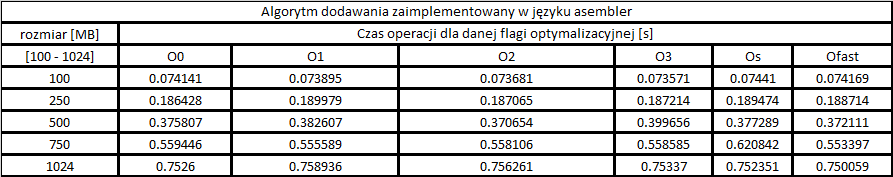
\includegraphics[scale=0.65]{charts/add_asm.png}

\end{figure}

\begin{figure}[h!]
\centering
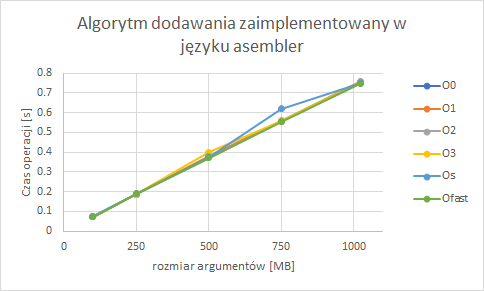
\includegraphics[scale=0.75]{charts/add_asm_p.png}

\end{figure}

\vspace{5mm}

Powyższy wykres prezentuje zależność czasową dla funkcji zaimplementowanej w języku asembler, która realizuje dodanie dwóch zadanych liczb w postaci tablicy bajtów z wykorzystaniem instrukcji \textit{adc}. Powyższe badanie miało na celu sprawdzenie algorytmu bez procesu skalowania argumentów. Otrzymane wynik potwierdzają teorię, która głosi, że operacja dodawania zależna jest od wielkości operandów i wraz ze wzrostem rozmiarów składników czas operacji rośnie. Należy również zauważyć, że zastosowanie różnych flag optymalizacyjnych w niewielkim stopniu wpływa na czas wykonania algorytmu. Spowodowane jest to implementacją całej funkcji w języku asemblera, co powoduje brak możliwości optymalizacji kodu przez \textit{gcc}. Stosunkowy długi czas wykonywania operacji spowodowany jest również implementacją algorytmu, gdzie w każdej iteracji dodawany jest bajt po bajcie. Pierwszym krokiem jaki należałoby podjąć aby zoptymalizować algorytm jest dodawanie ośmiu bajtów w każdej iteracji, dzięki czemu osiągnęlibyśmy przynajmniej ośmiokrotnie lepszy rezultat.

\newpage{}

\begin{figure}[h!]

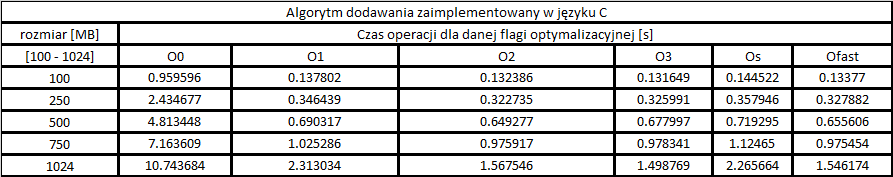
\includegraphics[scale=0.65]{charts/add_c.png}

\end{figure}

\begin{figure}[h!]
\centering
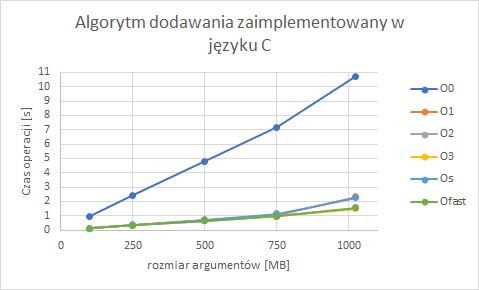
\includegraphics[scale=0.75]{charts/add_c_p.png}

\end{figure}

\vspace{5mm}

Analizę naiwnej implementacji w języku \textit{C} przeprowadziliśmy w celu pokazania różnicy pomiędzy czasem wykonywania algorytmu wykorzystującego instrukcje asemblera a tym zdefiniowanym w języku \textit{C}. Dane przedstawione w formie tabelarycznej pokazują znaczącą różnicę pomiędzy czasami wykonania operacji. Ponieważ całość algorytmu zdefiniowana jest w języku \textit{C}, na wykresie widzimy znacząco skrócony czas wykonywania dla flag odpowiadających wyższym stopniom optymalizacji. Zauważyć należy również, że pomimo znaczącej różnicy w czasie pomiędzy implementacją w języku \textit{C} a asemblerem, kolejne czasy dla większych operandów nie odbiegają od siebie tak bardzo jak w przypadku pierwszego algorytmu.
Główną wadą tego rozwiązania jest brak wykorzystania instrukcji \textit{adc}, która znacznie przyśpiesza proces dodawania i rozwiązuje problem propagacji przeniesienia na dalsze pozycje.

\newpage{}

\begin{figure}[h!]

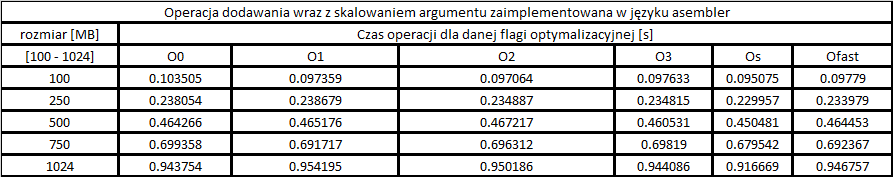
\includegraphics[scale=0.65]{charts/add_scale_asm.png}

\end{figure}

\begin{figure}[h!]
\centering
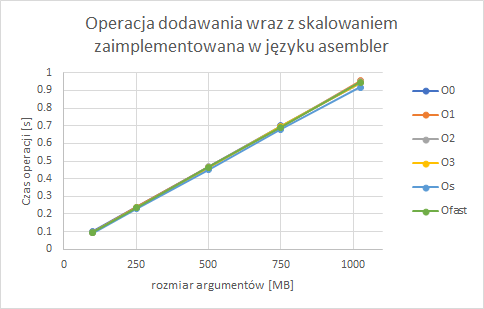
\includegraphics[scale=0.75]{charts/add_scale_asm_p.png}

\end{figure}

\vspace{5mm}

Wykres nie odbiega znacznie od tego prezentującego zależność dla samego algorytmu dodawania. Ponieważ tylko jeden z argumentów musi być skalowany do rozmiaru wyniku, wykorzystując funkcję \textit{memcpy} znacznie zmniejszyliśmy czas wykonania operacji skalowania, dzięki czemu narzut czasu jaki nakłada ona na sam algorytm wynosi około \textit{0.1 s}. Operacja skalowania napisana została w całości w języku \textit{C}, lecz jak widać na wykresie czas wykonania całej operacji w małym stopniu zależy od zastosowanej flagi optymalizacyjnej.

\newpage{}

\begin{figure}[h!]

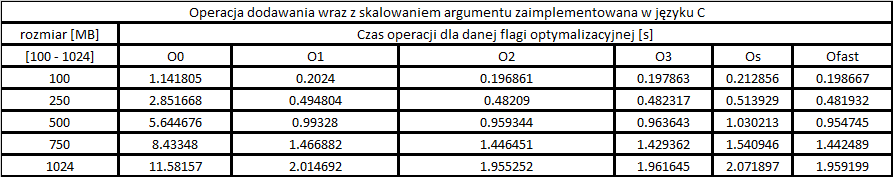
\includegraphics[scale=0.65]{charts/add_scale_c.png}

\end{figure}

\begin{figure}[h!]
\centering
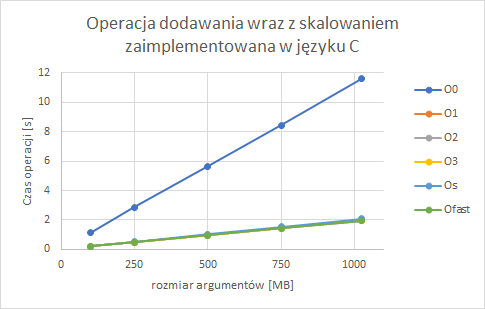
\includegraphics[scale=0.75]{charts/add_scale_c_p.png}

\end{figure}

\vspace{5mm}

Powyższy diagram pokazuje zależność czasową algorytmu dodawania wraz z narzutem funkcji skalującej pierwszy z składników do rozmiaru wyniku. Cały algorytm napisany został w języku \textit{C}, dzięki czemu zaobserwować możemy znacznie krótszy czas wykonania dla wyższych flag optymalizacyjnych. Pomimo większej optymalizacji zapewnionej przez kompilator \textit{gcc} czas wykonania całej operacji jest znacząco dłuższy od algorytmu zaimplementowanego z użyciem instrukcji \textit{adc}. Tak jak wcześniej narzut funkcji odpowiedzialnej za skalowanie jest niewielki w porównaniu do czasu potrzebnego do obliczenia wyniku. 

\newpage{}

\subsubsection{Operacja odejmowania}

\begin{figure}[h!]

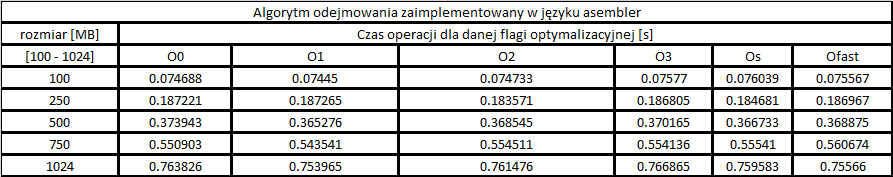
\includegraphics[scale=0.65]{charts/sbb_asm.png}

\end{figure}

\begin{figure}[h!]
\centering
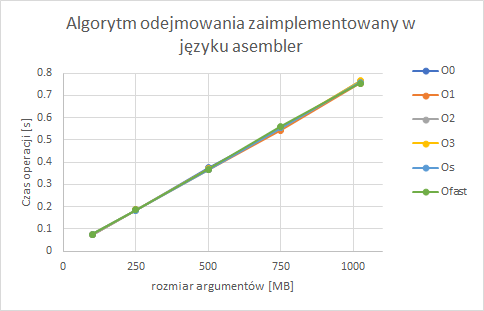
\includegraphics[scale=0.75]{charts/sbb_asm_p.png}

\end{figure}

\vspace{5mm}

Algorytm odejmowania został zaimplementowany analogicznie do instrukcji wykorzystanych w operacji dodawania z tym, że zamiast instrukcji \textit{adc} wykorzystano mnemonik \textit{sbb}. Potwierdzają to również dane w tabeli oraz wykres, gdzie wyniki zbliżone są do tych otrzymanych podczas badania algorytmu dodawania. Całość algorytmu zrealizowana została w języku asemblera w związku z czym optymalizacja zapewniana przez kompilator \textit{gcc} nie poprawia znacznie czasów operacji.

\newpage{}

\begin{figure}[h!]

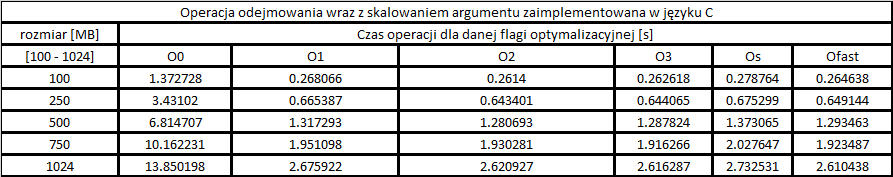
\includegraphics[scale=0.65]{charts/sbb_scale_c.png}

\end{figure}

\begin{figure}[h!]
\centering
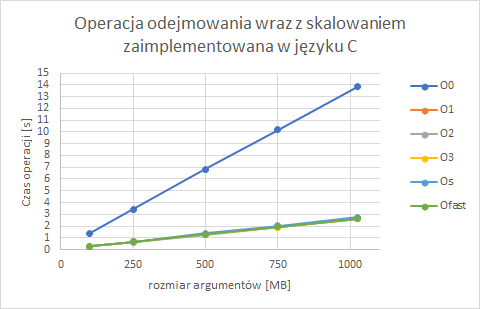
\includegraphics[scale=0.75]{charts/sbb_scale_c_p.png}

\end{figure}

\vspace{5mm}

Operacja odejmowania w języku \textit{C} zrealizowana została z wykorzystaniem zależności:

\begin{equation}
\bar{X} - \bar{Y} = X + \underline{Y} = X + \bar{Y} + ulp
\end{equation}

Algorytm polegał na zanegowaniu każdego z bitów drugiego z operandów a następnie dodanie jedynki na najmniej znaczącej pozycji. Kolejnym krokiem było wykorzystanie naiwnej implementacji dodawania w języku \textit{C} na odjemnej oraz wcześniej wyznaczonym odjemniku. Sposób ten był bardzo nieefektywny, ponieważ W pierwszym kroku należało przejrzeć całą tablicę i zanegować każdą pozycję w tablicy, która przechowuje drugi składnik odejmowania. Następnie dodawano jedynkę na najmniej znaczącej pozycji, bez wykorzystania instrukcji \textit{adc}, przez co analogicznie należało przejrzeć całą tablicę w celu zapewnienia poprawnej propagacji przeniesienia. Rezultat wykonania wszystkich zdefiniowanych wyżej operacji, służących do poprawnego obliczenia wyniku widoczny jest na wykresie oraz w tabeli, gdzie czas jest znacząco dłuższy od czasu wykonania sumowania. Algorytm ten jest znacząco mniej wydajny od tego zaimplementowanego z użyciem instrukcji \textit{sbb}, nawet po uwzględnieniu optymalizacji zapewnianej przez \textit{gcc}.

\newpage{}

\begin{figure}[h!]

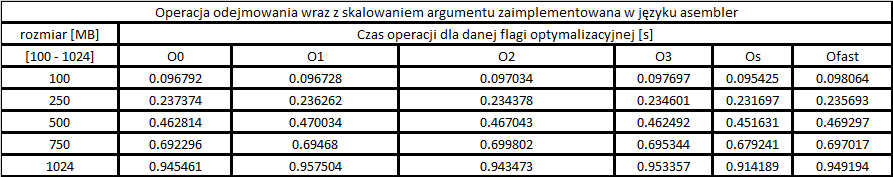
\includegraphics[scale=0.65]{charts/sbb_scale_asm.png}

\end{figure}

\begin{figure}[h!]
\centering
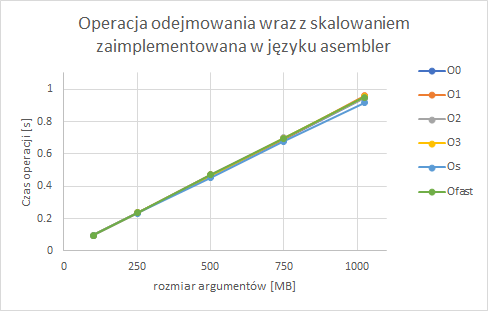
\includegraphics[scale=0.75]{charts/sbb_scale_asm_p.png}

\end{figure}

\vspace{5mm}

Tak jak w przypadku algorytmu dodawania, proces skalowania argumentu do rozmiaru wyniku zapewnia narzut o średniej wartości \textit{0.2 s} na czas wykonywania operacji. W porównaniu do algorytmu zaimplementowanego w języku \textit{C} wypada on znacznie lepiej, pomimo znikomej optymalizacji ze strony kompilatora. Dane zaprezentowane na wykresie oraz w tabeli potwierdzają analogiczne implementację algorytmu odejmowania oraz dodawania, ponieważ poszczególne czasy wykonania dla operandów o równych wielkościach nie odbiegają od siebie znacząco.

\newpage{}

\subsubsection{Operacja mnożenia}

\begin{figure}[h!]

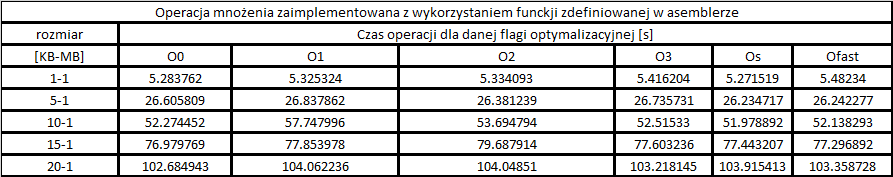
\includegraphics[scale=0.65]{charts/mul_asm.png}

\end{figure}

\begin{figure}[h!]
\centering
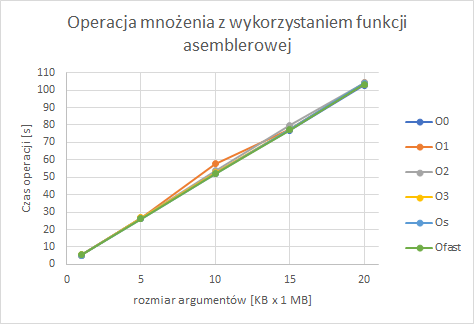
\includegraphics[scale=0.75]{charts/mul_asm_p.png}

\end{figure}

\vspace{5mm}

Mnożenie znacznie przekracza czasy wykonywania wszystkich poprzednich implementacji, ponieważ jest operacją, która wymaga największego nakładu pracy w celu wyznaczenia całego iloczynu. Aby uzyskać ostateczny wynik wyznaczyć należy wszystkie iloczyny częściowe a następnie odpowiednio je posumować, co przekłada się na czasy widoczne w tabeli oraz na wykresie. Aby wykorzystać instrukcję \textit{mul}, zdefiniowaliśmy funkcję w języku asemblera, która odpowiedzialna jest za przemnożenie kolejnego bajta mnożnika przez całą mnożną oraz odpowiednie posumowanie uzyskanych iloczynów z obecnym iloczynem wynikowym. Skutkuje to słabą optymalizacją ze strony \textit{gcc}, lecz zapewnia większą wydajność niż algorytm zaimplementowany w czystym języku \textit{C}. Mnożna oraz mnożnik zostały odpowiednio dobrane tak aby zapewnić sensowny czas wykonania operacji oraz pokazać zależność pomiędzy kolejnymi czasami egzekucji algorytmu oraz wielkością operandów.


\newpage{}

\subsubsection{Operacja dzielenia}

\begin{figure}[h!]

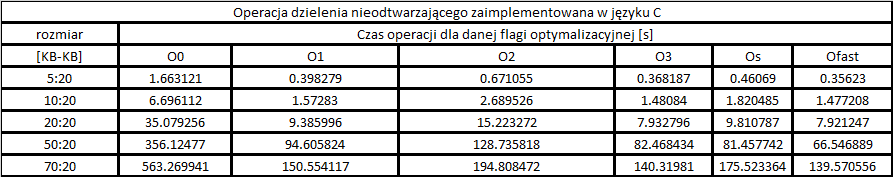
\includegraphics[scale=0.65]{charts/divide_c.png}

\end{figure}

\begin{figure}[h!]
\centering
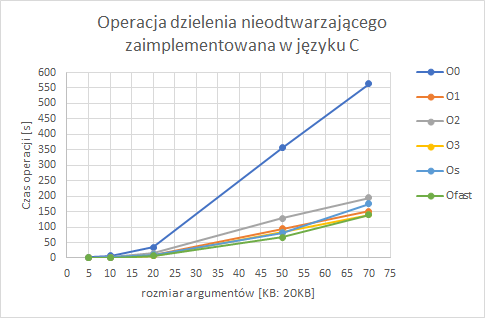
\includegraphics[scale=0.75]{charts/divide_c_p.png}

\end{figure}

\vspace{5mm}

Aby zapewnić odpowiednią skalowalność algorytmu, cała operacja zrealizowana została jako iteracyjne odejmowanie odpowiednio wyskalowanego dzielnika. Całość algorytmu napisana została w języku \textit{C}, dzięki czemu wraz z kompilacją z wyższymi stopniami optymalizacji zauważyć możemy, istotnie zmniejszający się czas obliczenia ilorazu. Pomimo braku wykorzystania instrukcji \textit{div}, algorytm poprawnie realizuje swoje zadanie, oraz osiąga względnie akceptowalny czas wykonania dla małych operandów. Porównując otrzymane wynik z rezultatem badań poprzednich algorytmów, zauważyć można, że zaproponowana przez nas implementacja dzielenie nie charakteryzuje się liniową zależnością tak jak wcześniejsze operacje. Spowodowane jest to dużym narzutem czasowym wprowadzonym przez operację skalowania dzielnika podczas kolejnych iteracji algorytmu oraz wykonanie dużej liczby odejmowań w celu wyznaczenie ilorazu. Algorytm bazuje również na wcześniej zaimplementowanych operacjach dodawania i odejmowania, w związku z czym zaproponowana poprawa wcześniej wymienionych algorytmów wpłynęłaby również na poprawę wydajności dzielenia.

\newpage{}

\section{Profilowanie oraz analiza pamięciowa}

W celu dokładnej analizy zaimplementowanych algorytmów posłużono się narzędziem \textit{Gprof}, które umożliwia profilowanie wykonywanego kodu programu. Wynikiem wykorzystania narzędzia jest raport w którym pokazane jest jaka część wykonywanych instrukcji była najbardziej czasochłonna oraz które z nich były najczęściej wykonywane. Następnie wykorzystano dostępne flagi kompilatora: \textit{-fsanitize} oraz \textit{-fno-omit-frame-pointer}, dzięki którym zlokalizowano miejsca w programie w których zabrakło deaalokacji wcześniej zajętych obszarów. Ostatecznie plik wykonywalny, który testował wszystkie funkcje oferowane przez bibliotekę został poddany analizie z użyciem narzędzia \textit{valgrind} aby przeprowadzić dokładną analizę pamięciową oraz zorientować się jak wiele pamięci wykorzystuje program podczas swojego działania. 

\subsection{Profilowanie przy użyciu narzędzia $Gprof$}

Poniżej zamieszczono przykładowy kod programu, testujący wszystkie funkcje dostarczane przez bibliotekę, gdzie operandami danych metod są liczby o największych rozmiarach użytych podczas badania algorytmów. Wielkość argumentów jest kluczowa, ponieważ znacząco wpływa na czas egzekucji programu, dzięki czemu podczas profilowania możemy zaobserwować najbardziej czasochłonne operacje. Profilowanie przeprowadzone zostało bez optymalizacji dostarczanej przez kompilator \textit{gcc} w celu uwidocznienia różnicy w czasie wykonywania danych algorytmów.

\newpage

\begin{minted}{C}
#include "EfficiencyTests.h"

int main()
{
    TCNumber *firstNumber = getNumberFromBinaryFile(firstNumber1GBPath, 0);
    TCNumber *secondNumber = getNumberFromBinaryFile(secondNumber1GBPath, 0);
    TCNumber *result;

    // Run add operation
    result = add(firstNumber, secondNumber);
    delete (result);

    // Recreate structures
    firstNumber = getNumberFromBinaryFile(firstNumber1GBPath, 0);
    secondNumber = getNumberFromBinaryFile(secondNumber1GBPath, 0);

    // Run subtraction operation
    result = subtract(firstNumber, secondNumber);
    delete (result);

    // Files for multiplication
    firstNumber = getNumberFromBinaryFile(firstNumber1MBPath, 0);
    secondNumber = getNumberFromBinaryFile(firstNumber20KBPath, 0);

    // Test multiplication algorithm
    result = multiply(firstNumber, secondNumber);
    delete (result);

    // Files for division
    firstNumber = getNumberFromBinaryFile(secondNumber50KBPath, 0);
    secondNumber = getNumberFromBinaryFile(firstNumber20KBPath, 0);

    result = divide(firstNumber, secondNumber, 0);
    delete (result);

    return 0;
}

\end{minted}

\clearpage{}

% OUTPUT Z PROFILOWANIA (MOŻE BYĆ SCREEN Z TERMINALA JAK TO SIĘ UŁOŻYŁO)
Poniższa tabela przedstawia wynik profilowania powyższego programu wraz z wszystkimi informacja dostarczonymi przez narzędzie \textit{Gprof}. Tabela prezentuje rozkład czasu ze względu na wykonywania funkcje oraz ilość ich wywołań.

\begin{figure}[h!]
\centering
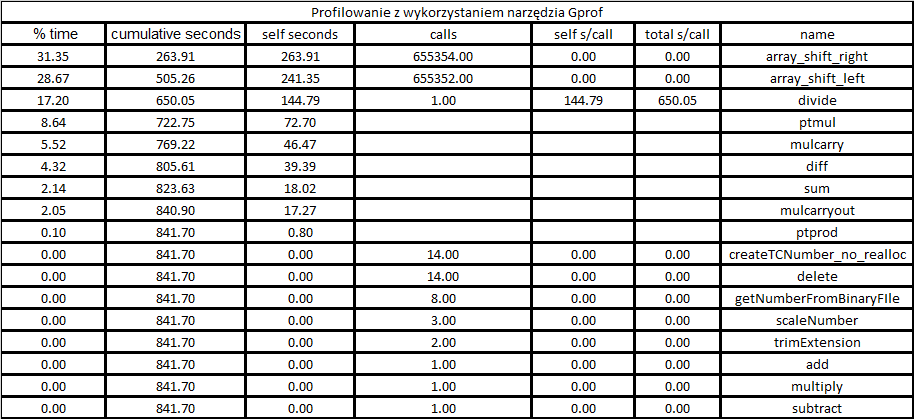
\includegraphics[scale=0.60]{charts/GprofTable.png}

\end{figure}

\begin{itemize}
    \item Kolumna \textit{\% time} prezentuje ilość czasu wyrażoną w procentach w stosunku do całego czasu wykonywania programu.
    \item \textit{Cumulative seconds} zawiera ilość sekund przeznaczonych na wykonanie wszystkich funkcji, które znajdują się na daną metodą w tabeli wraz z czasem wykonania funkcji w danym wierszu.
    \item \textit{Self seconds} pokazuje czas wykonywania konkretnej funkcji wyrażony w sekundach.
    \item Kolumna \textit{Calls} oznacza ilość wywołań danej funkcji.
    \item \textit{Self s/call} prezentuje średnią ilość sekund wykonania danej metody przypadającej na jedne wywołanie funkcji.
    \item \textit{Total s/call} zawiera średni czas wykonania funkcji wraz z wszystkimi metodami, które dana funkcja wykonuje z swojego ciała.
    \item \textit{Name} zawiera nazwę funkcji, której dotyczą dane w danym wierszu.
\end{itemize}

Analizując powyższą tabelę, możemy wyciągnąć wnioski na temat najbardziej czasochłonnych procesów, które odbywają się podczas egzekucji programu dzięki czemu otrzymujemy informacje, które algorytmy wymagają optymalizacji. W powyższej tabeli widzimy, że operacja dzielenie jest zdecydowanie najbardziej czasochłonna, ponieważ zrealizowana została jako iteracyjne odejmowanie wyskalowanego dzielnika oraz odpowiednie przesuwanie rezultatu, które zajmuje zdecydowaną większość czasu. Operacja mnożenia wykorzystuje instrukcję \textit{mul}, dzięki czemu osiąga lepszy czas wykonywania całego algorytmu w stosunku do algorytmu dzielenia. Etykiety \textit{ptmul, mulcarry, diff, sum, mullcarryout} oraz \textit{ptprod} definiują miejsca w kodzie asemblerowym, gdzie realizowane są kluczowe operacji potrzebne do wykonania danego algorytmu. Natomiast funkcje \textit{add, multiply, subtract} są jedynie metodami zdefiniowanymi w języku \textit{C}, które odpowiadają za przygotowanie argumentów do algorytmu zdefiniowanego w języku asemblera w związku z czym zajmują znikome ilości czasu. 

Poniżej zamieszczono drzewo wywołań programu, które posortowane zostało ze względu na czas wywołania każdej z funkcji.


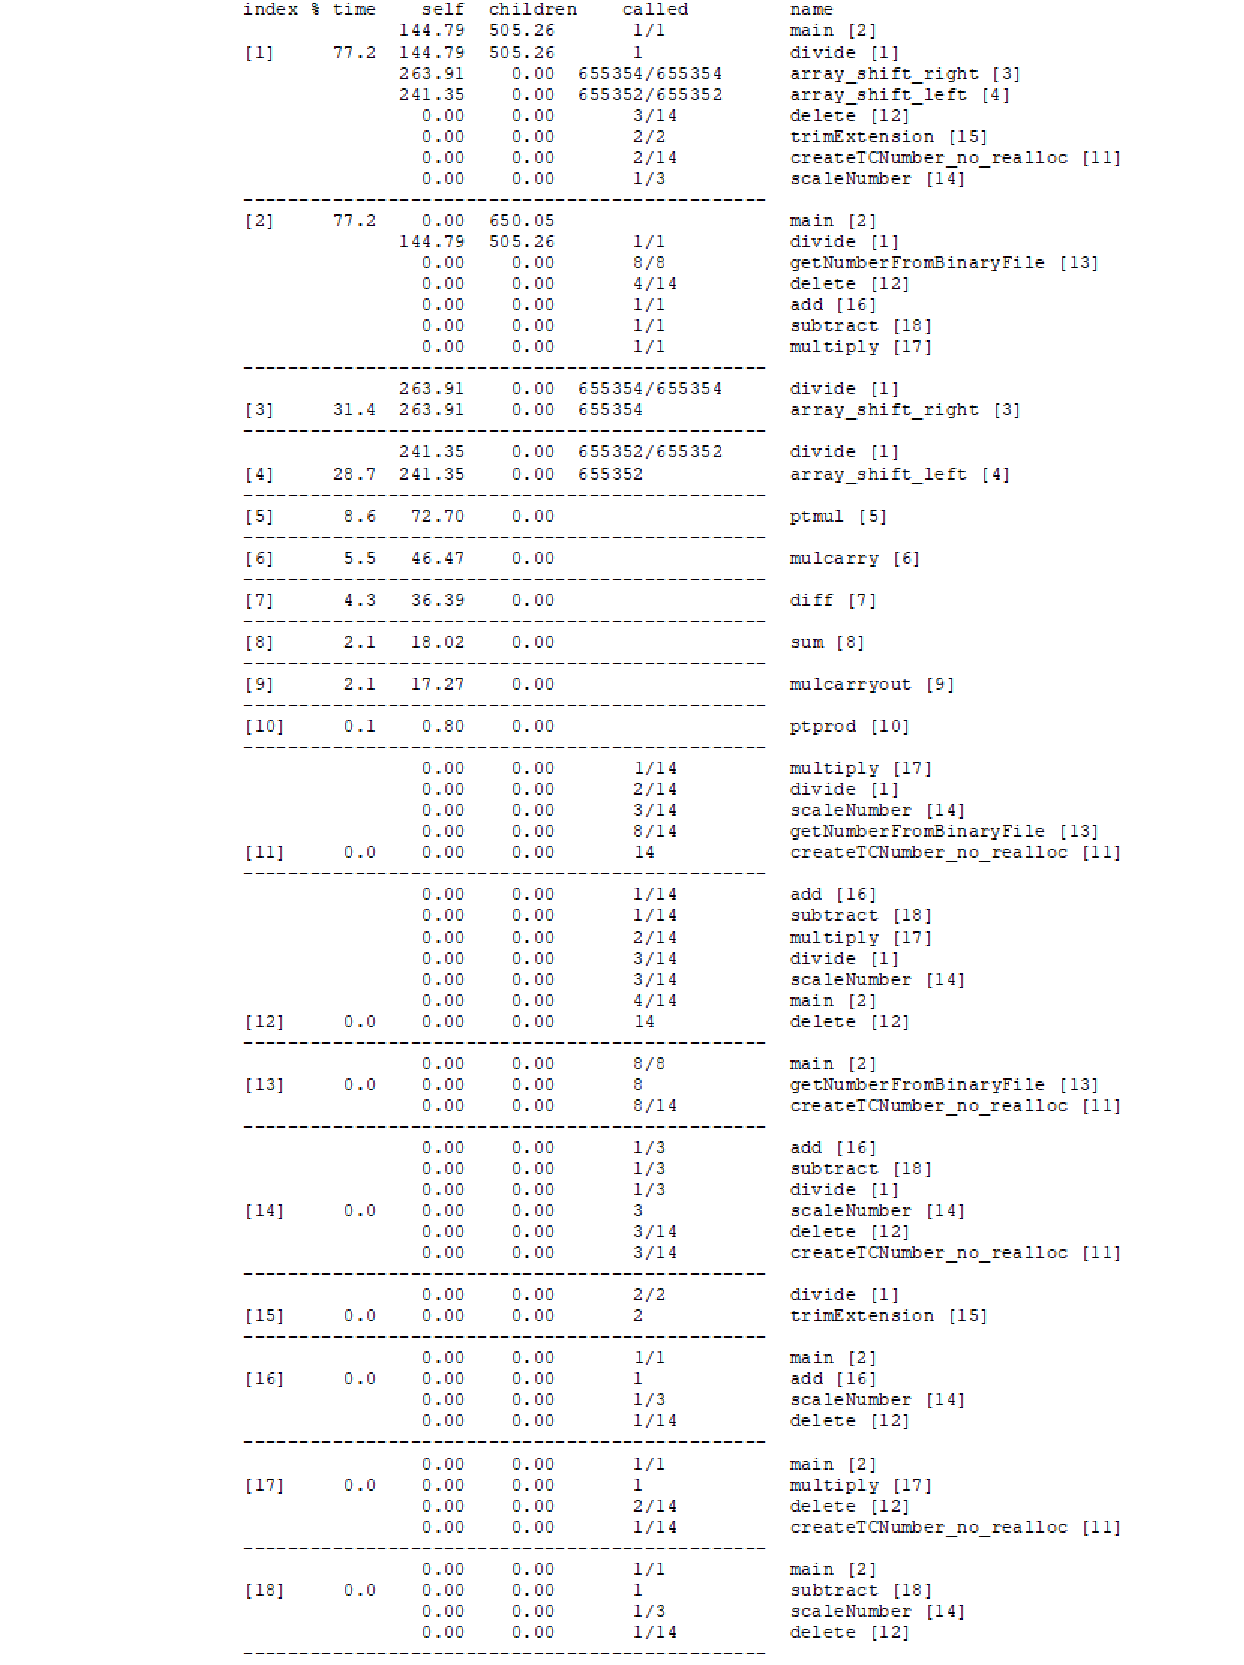
\includepdf{Call-Tree-Gprof.pdf}

Drzewo również obrazuje wnioski, które zaprezentowane zostały w poprzednim akapicie. Krokami, które podjąć należy w celu optymalizacji działania biblioteki jest próba zmniejszenia liczby wywołań funkcji \textit{array\_shift\_right} oraz \textit{array\_shift\_left}, które zajmują zdecydowaną większość czasu działania programu. Podczas analizy algorytmów pod każdym z wykresów zamieszczono sugestie, które wykorzystać można podczas optymalizacji danych algorytmów, co wpłynęłoby również na wyniki kolejnego profilowania. Statyczna analiza kodu pozwala na dokładną analizę czasową wykonywanych algorytmów oraz dostarcza przydatnych informacji na temat ilości wywołań danych funkcji.


\subsection{Wykorzystanie narzędzia \textit{Valgrind} oraz flagi \textit{-fsanitize} do detekcji wycieków pamięci}

Flagi \textit{-fsanitize=address} oraz \textit{-fno-omit-frame-pointer} okazały się kluczowe podczas implementacji algorytmu dzielenia, ponieważ wymaga on dużej liczby operacji na pamięci, a zastosowane flagi pozwoliły na dynamiczną analizę wykonywanego kodu, dzięki czemu na bieżąco lokalizowaliśmy błędne adresowanie oraz wycieki pamięci. Flagi pozwalające na dynamiczną analizę kodu w połączeniu z flagą \textit{-g}, prezentowały dokładną linię kodu w której występował dany błąd, dzięki czemu szybko lokalizowaliśmy naruszenie pamięci. 

Następnie po pozbyciu się wszystkich problemów związanych z zarządzaniem pamięcią wykorzystaliśmy program \textit{Valgrind}, który prezentował dokładniejsze informacje dotyczące zarządzania pamięcią. 

Poniżej zaprezentowano wynik działania programu wraz z jego podsumowaniem dostarczonym przez analizator.

\begin{figure}[h!]

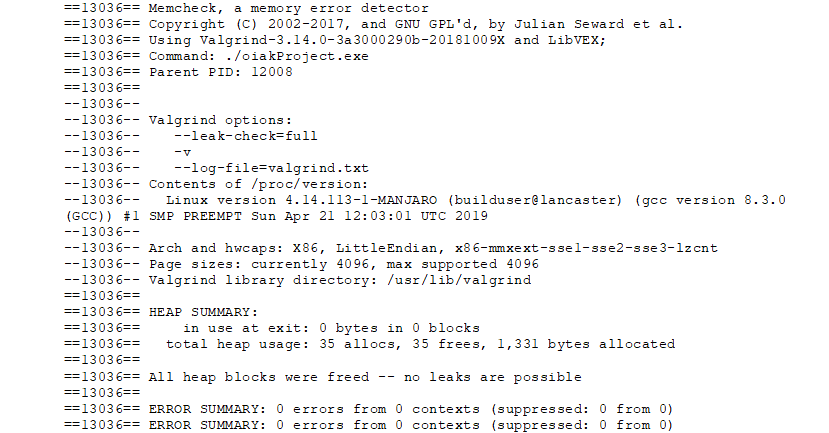
\includegraphics[scale=0.6]{charts/valgrind.png}

\end{figure}

Analiza pamięciowa przeprowadzona została na programie, który wykorzystywał wszystkie funkcje oferowane przez bibliotekę, dzięki czemu mamy pewność, że wykonywany kod nie zawiera miejsc w których dochodzi do wycieku pamięci. Dynamiczny analizator kodu pozwolił wykryć błędy w alokacji, pokazał błędy podczas wykorzystania funkcji \textit{memcpy} oraz pomagał podczas debugowania kodu, który wykonywał wiele operacji na stercie.

\clearpage

\section{Wnioski reasumujące cały projekt}

Główne cele projektu zostały zrealizowane zgodnie z założeniami zdefiniowanymi na początku semestru. Biblioteka napisana w języku \textit{C} oferuje cztery podstawowe operacje arytmetyczne, operujące na liczbach dowolnej precyzji. 

Wybór wewnętrznej reprezentacji \textit{U2}, był bardzo trafny, ponieważ reprezentacja ta jest używana przez język asemblera, dzięki czemu nie musieliśmy przeprowadzać dodatkowych operacji w celu wykorzystania ich podczas operacji na mnemonikach. 

W projekcie silnie polegaliśmy oraz wykorzystywaliśmy łatwość łączenia kodu języka \textit{C} z kodem asemblerowym, aby możliwe najlepiej zoptymalizować dane algorytmy. Implementacja głównych algorytmów w języku asemblera przełożyła się na optymalizację zapewnianą przez \textit{gcc}, co widoczne jest na wykresach, gdzie flagi optymalizacyjne dla funkcji napisanych w asemblerze nie odgrywają wielkiej roli. Pomimo to algorytmy te znacznie przewyższają wydajnością naiwne implementacje w języku \textit{C}, które napisaliśmy na początku zajęć.

Kluczowym elementem projektu było wykorzystanie w projekcie biblioteki \textit{Unity}, która pozwoliła nam na pełne pokrycie testami każdej z operacji oraz zapewniała poprawność danych operacji podczas ewentualnej zmiany algorytmu. Testy jednostkowe pozwoliły nam na bieżąco sprawdzać poprawność danych algorytmów,, dzięki czemu szybciej dochodziliśmy do rozwiązania problemu.

Ostatni etap dotyczył aspektu badawczego zaimplementowanych algorytmów. Ponieważ podczas pierwszych prób implementacji nie do końca zrozumieliśmy zamysł wykorzystania instrukcji asemblerowych, które służyć miały poprawie wydajności algorytmów, stworzyliśmy funkcje, które poprawnie realizowały dane zadanie lecz robiły to w sposób niewydajny. Naiwne implementacje odłączyliśmy od głównego projektu, ale wykorzystaliśmy je podczas przeprowadzania badań w celu pokazania różnicy pomiędzy danymi algorytmami. Cały przebieg eksperymentu został udokumentowany w sprawozdaniu, poprzez wykresy oraz tabele z danymi wraz z płynącymi z tych danych wnioskami.

Realizowany temat dobrze nakreślił nam problem reprezentacji liczb w pamięci komputera oraz wyzwania dotyczące zapewnienia dowolnej precyzji wykonywanych operacji. Istotnym elementem projektu był sposób reprezentacji liczb, ponieważ definiował on później wykonywane operacje. Wykorzystując strukturę do reprezentacji liczby, która przechowuje rozmiar liczby, daną liczbę w systemie U2, oraz pozycję najmniej znaczącego bitu, rozwiązaliśmy problem odpowiedniego skalowania liczby oraz odpowiedniego wyznaczania jej pozycji podczas wykonywania danych operacji.



\newpage

\begin{thebibliography}{9}

\bibitem{Zak}
Materiały dostępne na stronie zakładu architektury komputerów 
\\\texttt{http://zak.ict.pwr.wroc.pl/}

\bibitem{Unity} 
ThrowTheSwitch, Unity
\\\texttt{http://www.throwtheswitch.org/unity}
\\\texttt{https://github.com/ThrowTheSwitch/Unity}
 
\bibitem{Valgrind} 
Valgrind
\\\texttt{http://www.valgrind.org/}

\bibitem{Travis-CI} 
Travis CI
\\\texttt{https://docs.travis-ci.com}
\end{thebibliography}


\end{document}
